\documentclass[12pt,a4paper]{article}
\usepackage[spanish]{babel} % espanol
\usepackage[utf8]{inputenc} % acentos sin codigo
\usepackage[left=3.5cm,right=2cm,top=2.5cm,bottom=2cm,includehead,includefoot]{geometry}  %margenes segun pauta de la U
\usepackage{setspace}
\onehalfspacing %interlineado 1.5
\usepackage{graphicx}
\usepackage[usenames]{color}
\usepackage{amsfonts}
\usepackage{algpseudocode}
\usepackage{amsmath}
\usepackage{booktabs} %Rules en las tablas
\usepackage{listings}
\usepackage{xcolor}
\usepackage{afterpage}
\usepackage{float}
\usepackage{subfigure}
\usepackage{verbatim} %Comentarios con \begin end comment
\usepackage{csquotes}
\usepackage{datetime} %Para obtener formato a la fecha
\usepackage[backend=bibtex,bibencoding=ascii,sorting=none]{biblatex}%packages Bibliografia
\bibliography{biblio}%se carga el archivo

\usepackage{times} %font times new roman (?)

\newcommand{\grad}{$^{\circ}$}

\let\stdsection\section
\renewcommand\section{\newpage\stdsection}


\newdateformat{fecha}{%Método para obtener el mes y el año
  \monthname[\THEMONTH] \THEYEAR}



\pagestyle{headings}

\begin{document}


\thispagestyle{empty}
\vspace*{-2cm}
\hspace{-3cm}
\hbox{\vsize = 5cm
\vbox{\hsize = 11cm
\begin{flushleft}
{\small{\bf UNIVERSIDAD CAT\'OLICA DEL MAULE}\\
Facultad de Ciencias de la Ingenier\'ia\\
Escuela de Ingenier\'ia Civil Inform\'atica}
\end{flushleft}}

\vbox{\hsize = 7cm
\begin{flushright}
{\small{\bf PROFESOR GU\'IA}\\
Mary Carmen Jarur\\
\hspace{1cm}}
\end{flushright}}
}
\vspace{5.5cm}

\begin{center}
	{\Large {\bf NOMBRE DE LA TESIS LOREM IPSUM DOLOR SIR AMET, CONSECTETUR ADIPISCING ELIT}}
	
\

\

\small {\bf H\'ECTOR GABRIEL PEREDO URBINA}\\


\

\

\textmd{Tesis para optar al\\ T\'itulo Profesional de Ingeniero Civil Inform\'atico}

\vspace{4cm}
\vfill{{\large {\sc Talca, \fecha\today }}}

\end{center} 

\pagebreak

%%%%%%%%%%%%%%%%%%%%% FIN  PORTADA     %%%%%%%%%%%%%%%%%%%%%%%%%%%


%%%%%%%%%%%%%%%%%%%%% PORTADA COMISION    %%%%%%%%%%%%%%%%%%%%%%%%

\thispagestyle{empty}

\begin{center}
    {\small {\bf UNIVERSIDAD CATÓLICA DEL MAULE}}\\
    \small {\bf FACULTAD DE CIENCIAS DE LA INGENIERÍA}\\
    \small {\bf ESCUELA DE INGENIERÍA CIVIL INFORMÁTICA}

\end{center}
\vspace{1cm}

\begin{center}
{\small {\bf TESIS PARA OPTAR AL}}\\
\small {\bf AL TÍTULO PROFESIONAL DE INGENIERO CIVIL INFORMÁTICO}\\
\end{center}

\vspace{1cm}

\begin{center}
\bf  {NOMBRE DE LA TESIS LOREM IPSUM DOLOR SIR AMET, CONSECTETUR ADIPISCING ELIT}

\

\small {\bf  HECTOR GABRIEL PEREDO URBINA}\\

\end{center}

\vspace{1cm}

\begin{tabular}{l@{\hspace{1cm}}c@{\hspace{3cm}}l@{\hspace{1cm}}l}
{\bf COMISI\'ON EXAMINADORA}&&{\bf FIRMA}&\\
&&&\\
PROFESOR GUÍA &&&\\
MARY CARMEN JARUR MUÑOZ&&&\\
\cline{2-3}
&&&\\

PROFESOR COMISI\'ON&&& \\
DR. HERNAN MAUREIRA P&&&\\
\cline{2-3}
&&&\\

PROFESOR COMISI\'ON&&& \\
DR. MARCO MORA&&&\\
\cline{2-3}
&&&\\

&&&\\
NOTA FINAL EXAMEN DE T\'ITULO &&& \\
\cline{2-3}
\end{tabular}
\vspace{.7cm}


\begin{center}
\vfill{{\large {\sc Talca, \fecha\today }}}
\end{center}


\pagebreak

%%%%%%%%%%%%%%%%%%%%% FIN  PORTADA COMISION   %%%%%%%%%%%%%%%%%%%%%%



\tableofcontents %Indice de Contenidos
\thispagestyle{empty}
\pagebreak



\section{Introducción}
La comprensión de las dinámicas y patrones de movimiento humano, se facilitan enormemente con el apoyo de tecnologías adecuadas, que permitan medir, registrar y analizar variables cinemáticas. Particularmente, el estudio del movimiento humano (Kinesiología) depende hoy en día de las facilidades tecnológicas que ofrece la electrónica (sensores, microcontroladores, sistema de adquisición de señales) y las ciencias de la computación (procesamiento, análisis y posterior reporte adecuado de  variables cinemáticas y cinéticas).  
Las soluciones tecnológicas que hoy existen, no solo permiten realizar el seguimiento (‘tracking’) y representación gráfica, sino que además facilitan la representación en tiempo real de las variables de interés, conformando con esto los denominados sistemas de Bio-feedback (retroalimentación de señales biológicas). Aunque existen alternativas adecuadas para estos fines, poseen el inconveniente en lo prohibitivo de su valor comercial {\color{red} y a su vez las soluciones son cerradas, lo que limita}.
Frente a este desafío, está la posibilidad de integrar tecnología para conseguir soluciones de menores costos, que permitan realizar investigación y al mismo tiempo explorar posibilidades de innovación tecnológica que den paso al desarrollo de tecnología nacional.
Particularmente, este proyecto propone desarrollar un sistema de integración hardware-software que permita el registro del comportamiento pendular de la posición bípeda quieta (variables de posición y velocidad angular en el tiempo), habilitando funciones de bio-feedback que permitan replicar evaluaciones de balance postural.

\subsection{Objetivos Generales}
Diseñar e implementar un prototipo de software-hardware basado en un microcontrolador Arduino y un sensor de velocidad angular y acelerometría de 3 ejes, para el registro y representación gráfica del centro de masa y bio-realimentación.

\subsection{Objetivos Específicos}
\begin{itemize}
\item Integrar microcontrolador Arduino con sensor (giroscopio-acelerómetro).
\item Diseñar sistema que permita el registro y visualización de todas las variables cinemáticas (posición y velocidad angular) del centro de masa. 
\item Construcción de un sistema que facilite mediante bio-realimentación la posición del centro de presión (proyección del centro de masa).
\end{itemize}	

\subsection{Contribución Esperada}

El desarrollo del sistema permitirá medir y registrar el comportamiento del centro de masa y su respectiva proyección (centro de presión) durante la posición bípeda quieta, al mismo tiempo que realimentará la señal como mecanismo de evaluación de balance postural e implementación de biofeedback.

El principal alcance de la propuesta es la posibilidad de contar con una solución abierta, que facilita la importación de todos los registros además del procesamiento de las señales recogidas de las evaluaciones, permitiendo además integrar la solución a otros sistemas.
 
El costo del sistema, respecto a las soluciones de mercado (Biodex- Balance SD), es bajo, lo que le da viabilidad económica al proyecto, permitiendo además dejar el prototipo en operación en el Laboratorio de Biomecánica. 

Desde el punto de vista disciplinar (Ciencias de la Ingeniería), este proyecto materializa trabajos de investigación y colaboración transdisciplinario entre la Facultad de Ingeniería y la Facultad de Salud de la UCM. Además posiciona a los Ingenieros Informáticos como profesionales capaces de adecuarse a diferentes contextos mediante soluciones tecnológicas.
\subsection{Organizaci\'on de la Tesis}



\section{Estado del Arte}




\section{Marco Te\'orico}

\subsection{Protocolo de Comunicación $\mathbf{\mathrm{I^2C}}$}

Las principales características del protocolo de Comunicación $\mathrm{I^2C}$ \cite{I2C} son:
\begin{itemize}
\item Solo dos líneas para la comunicación son necesarias; una línea para la información serial (SDA) y otra para el reloj serial (SCL).
\item Cada dispositivo conectado al bus es direccionado por software por un ID único y usando relación Esclavo/Maestro todo el tiempo.
\item Posee un sistema de detección de colisiones lo que permite usar el modo multi-maestro previniendo la corrupción de los datos si dos o mas maestros comienzan a transferir datos de forma simultanea.
\item Serial, orientado en 8-bit ,transferencias de datos de forma bi-direccional pueden ser realizadas hasta los 100 kbit/s en el modo Estándar, hasta 400 kbit/s en el modo Rápido, hasta 1 Mbit/s en el MOdo Mas Rápido, o hasta 3.4 Mbit/s en el modo de Alta-Velocidad.
\item En el chip de filtrado se rechazan los picos en la línea de datos del bus de preservar la integridad de datos.

\begin{figure}[H]
	\centering
  	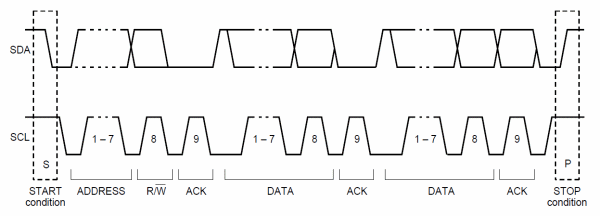
\includegraphics[width=0.9\textwidth]{images/Diagrama_I2C}
    \caption{Diagrama $\mathrm{I^2C.}$}
	\label{fig:diagramaI2C}
\end{figure}
\end{itemize}
\subsection{Sensores}

La Unidad de Medición Inercial MPU6050\cite{MPU6050} posee un Giroscópico y un Acelero-metro de 3 Ejes, el poseer estos 2 sensores de movimiento indica que existen almenos 6 grados de libertad para utilizar al momento de obtener las mediciones.

\begin{figure}[H]
  \centering
  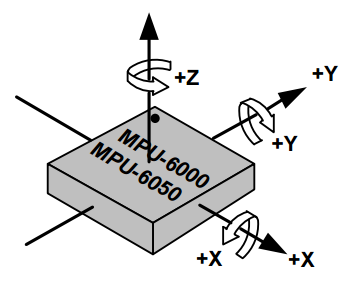
\includegraphics[scale=0.5]{images/MPU6050}
  \caption{Diagrama MPU6050}
  \label{fig:MPU6050}
\end{figure}

\subsection{Características Técnicas}

\begin{itemize}

\begin{table}[H]
  \centering
  \caption{Datos del Sensor}
  \begin{tabular}{|c|c|c|c|}
  \hline
  \multicolumn{2}{|c|}{Acelerómetro (g)} &\multicolumn{2}{|c|}{Giroscopio (\grad/seg)}   \\
  \hline
  Rango        & Sensibilidad   & Rango      & Sensibilidad \\ \hline
  $\pm 2g$     &  16384 & 250 \grad/seg  & 131      	\\ 
  $\pm 4g$     &  8192  & 250 \grad/seg  & 65.5      	\\
  $\pm 8g$     &  4096  & 250 \grad/seg  & 32.8      	\\
  $\pm 16g$    &  2048  & 250 \grad/seg  & 16.4      	\\ \hline
  \end{tabular}
\end{table}

\item \textbf{Rango: } Posee un rango configurable en los 2 sensores incluidos, tanto acelerómetro como giroscopio, el rango nos indica el dominio sobre el cual son obtenidos los datos, mas concretamente los valores máximos y mínimos que pueden ser obtenidos.
	
\item \textbf{Sensibilidad: }La sensibilidad describe la mínima variación medible, es decir la razón de cambio entre una variable entrante y el resultado de la variable saliente.

\item \textbf{Variables: } Las variables entregadas por el Acelerómetro consiste en la aceleración lineal percibida en cada eje expresada en veces de g, y en el Giroscopio corresponde  a la velocidad angular dada por la variación de los \grad/seg al girar sobre cada eje.

\item \textbf{Frecuencia de Muestreo: } La cantidad de datos que se pueden obtener en un intervalo de tiempo.

\item \textbf{Resolución: } Consiste en la mínima variación generada en los sensores que a su vez puede ser capturada por estos.

\end{itemize}

\subsection{Configuración de la IMU}
Para configurar los parámetros de la IMU la información debe ser configurada en cada uno de los registros internos presentes de esta. El mapa de los registros \cite{MAPREGISTER} proporcionado  en el sitio de InverSense.
\newline En la IMU se encuentran mas de 70 registros cada uno de 8 Bit, para la configuración se deben ser usados solo algunos pocos.
\begin{itemize}
\item \textbf{Configurar Frecuencia Muestreo:} Para obtener la cantidad de muestras que se obtendrán finalmente ``En Teoría'' se calcula usando la ecuación: 

\begin{equation} 
\label{eq:sampleratediv}
Sample Rate = \frac{Gyroscope Output Rate}{(1 + SMPLRT\_DIV) }
\end{equation}

this references the equation \ref{eq:sampleratediv}.
factores, tales como la velocidad del Puerto Serial pueden influir en el resultado, pero cambiando los datos almacenados en el registro \textbf{SMPRT\_DIV}, con los valores entre 0 y 255, el $Gyroscope Output Rate$ depende directamente del estado del filtro pasa-bajo, en caso de estar desactivado, el valor de $Gyroscope Output Rate$ seria 8Khz, en cambio si esta activado el $Gyroscope Output Rate$ tomaría el valor de 1Khz con lo cual haciendo los cálculos necesarios nos daría la formula teórica de que al tener desactivado el filtro pasa-bajo la frecuencia de muestreo varia entre las 8000 y 31 muestras/seg de forma teórica, al contrario en caso de estar activado el filtro, la fórmula para el calculo de la frecuencia de muestreo fluctuaría entre 1000 y 3.9 muestras/seg, por cada uno de los 6 datos obtenibles.

\item \textbf{Configurar Giroscopio:} El registro GYRO\_CONFIG para cambiar los Rangos de sensibilidad de el Giroscopio. Este registro para ser completado debe ser ingresado en los bits 3 y 4 del registro los valores en Binario 0,1,2,3 para configurar los cuatro rangos disponibles 250\grad/seg, 500\grad/seg, 1000\grad/seg y 2000\grad/seg. respectivamente.

\item \textbf{Configurar Acelerómetro:} De forma similar para configurar el Acelerómetro, solo que se usa el registro ACCEL\_CONFIG, se ingresan en los bits 3 y 4 del registro los valores en Binario 0,1,2,3 que representarán $\pm 2g$, $\pm 4g$, $\pm 8g$, $\pm 16g$ respectivamente.

\end{itemize}

\subsection{Obtención de los Datos (IMU)}
A partir de la configuración almacenada en los registros de la IMU,  se deben leer ciertos registros para la obtención de la información del movimiento registrado por los sensores inerciales:

\begin{itemize}
	\item \textbf{Obtención de la Velocidad Angular:} Para obtener la información proveniente del giroscópico, deben ser leídos 6 registros, $GYRO\_XOUT\_H$, $GYRO\_XOUT\_L$ , $GYRO\_YOUT\_H$, $GYRO\_YOUT\_L$, $GYRO_ZOUT\_H$, y $GYRO\_ZOUT\_L$ por cada eje medible son usados 2 registros de 8 bit, en donde luego de leer ambos registros del cada eje deben ser sumados para obtener el dato completo y ademas usar el complemento a 2, que genera como dato resultante un valor de entre aproximadamente $\pm 2^{15}$, el cual debe ser dividido según la sensibilidad asociada a el rango escogido, para obtener la información física.

\item \textbf{Obtención de la Aceleración:} Para obtener la información del  Acelerómetro al igual que en Giroscopio deben ser leídos los 6 pertenecientes a las mediciones $ACCEL\_XOUT\_H$ , $ACCEL\_XOUT\_L$ , $ACCEL\_YOUT\_H$, $ACCEL\_YOUT\_L$ , $ACCEL\_ZOUT\_H$, y $ACCEL\_ZOUT\_L$, en donde luego de unir los registros y usar el complemento a 2 acorde a cada eje, cada uno de estos valores deben ser dividido según el rango escogido, lo que determina la sensibilidad a usar, para obtener la información física.

\end{itemize}

 \subsection{Arduino IDE}
  Para la programación en la placa Arduino \cite{ARDUINO} se uso el IDE proporcionado por Arduino.
  

\subsection{QT Creator}
	El entorno de desarrollo (IDE) del Framework de C++ Qt  es Qt Creator en donde se incluyen las herramientas para la administación de los ficheros .h y .cpp usados en C++ junto con las opciones de compilación, ejecución y depuración del software.

\section{Desarrollo}
\subsection{Introducción}
\textcolor{red}{ Breve descripción de la solución completa, incluir esquemáticos}

A partir de balance y las ideas obtenidas en base a los estudios y resultados entregados por la plataforma de fuerza Kistler 9286b y balance SD se ideó una solución que opera de forma análoga a los que ya son utilizados en el laboratorio con un software que permita entregar información de manera similar a lo que entregan estos sistemas, para aprovechar los conocimientos de los actuales usuarios con el fin de disminuir la curva de aprendizaje del sistema implementado para que estos comprendan el software sin demasiado entrenamiento y a su vez la transición sea mas satisfactoria para estos.

El sensor inercial será puesto en el sujeto de prueba el cual captura la información del movimiento generado por el sujeto y lo trasmitirá al microcontrolador Arduino por el protocolo I2C en donde se recibe y traduce la información obtenida del sensor y el microcontrolador a su vez enviará mediante el puerto serial las muestras obtenidas, aceleración y velocidad angular en donde el software recibe la información y realiza el procesamiento para obtener el angulo junto con los análisis realizados \textcolor{red}{Agregar mas }

\begin{figure}[H]
\centering
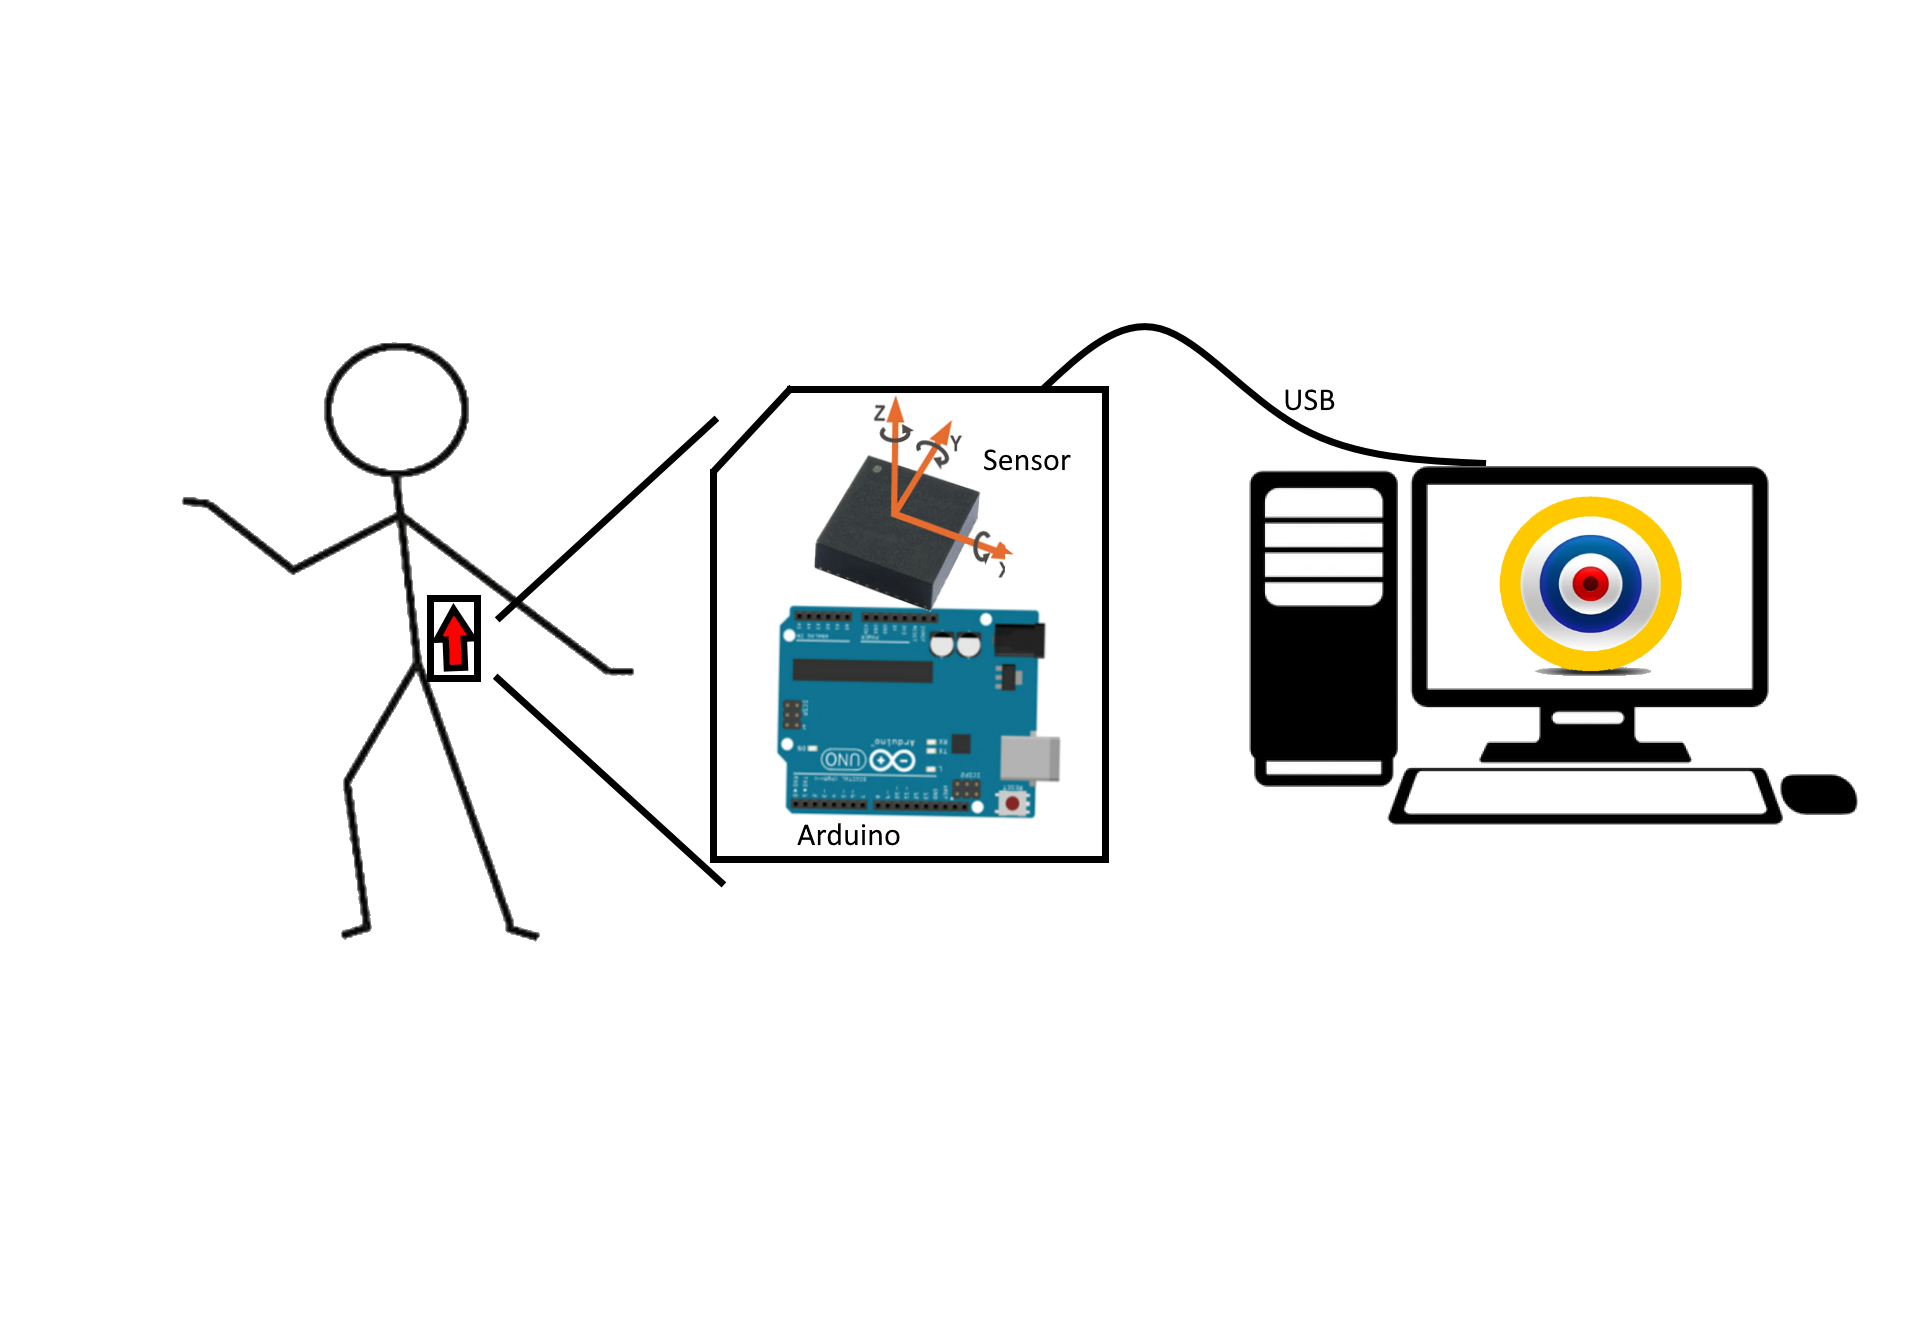
\includegraphics[scale=0.2]{images/diagrama_sistema}
\caption{Diagrama Sistema}
\label{fig:diagramasistema}
\end{figure}

\subsection{Configuración de Sensor}
Usando el IDE de Arduino se realiza la programación inicial del microcontrolador, en donde se configuran las direcciones de el IMU MPU6050 usadas, junto con la configuración inicial además de los datos desplegados por el puerto serial.
  En el Loop de ejecución se incluye la opción de configurar a Arduino, mediante la escritura de comandos en el puerto serial, para ajustar las configuraciones de los sensores a gusto del usuario ver Figura (\ref{fig:arduinocode}).

\begin{figure}[H]
\centering
	\includegraphics[scale=0.4]{images/diagramacodigoarduino}
	\caption{Diagrama Código Arduino}
	\label{fig:arduinocode}
\end{figure}
  
  Existen 4 parámetros a ser configurados de forma obligatoria Frecuencia de Muestreo, Filtro pasa bajo, rango Acelerómetro y  rango Giroscopio, antes de comenzar con la lectura de las de la información registros.
Para configurar los 4 parámetros requeridos debe ser recibida una cadena por el puerto serial en donde se analiza e interpretan los valores a utilizar para cada configuración. 
Una vez se completa la configuración se procede a la lectura de los registros para obtener los valores RAW acelerómetro como giroscopio para finalmente enviar mediante comunicación serial el valor resultante del dato RAW al ser dividido por la sensibilidad según el rango configurado.


\subsection{QT C++}
Para el desarrollo del software encargado de capturar y procesar la información proveniente de la comunicación serial entre la placa Arduino y el ordenador, se utilizara el Framework QT \cite{QT}, el cual esta basado en C++, por lo que en estabilidad y rendimiento es una de las mejores opciones a tener en consideración.
El usar un framework como Qt facilita en gran parte la creación de interfaces gráficas, cosa que C++ no trae por defecto, esto posibilita una integración rápida entre la parte lógica y visual del software a desarrollar.
La metodología usada para el desarrollo fue el método agiliza que al ser una solución de software con requisitos completamente definidos, mas que nada pautas del resultado esperado y ya que el programador pasa a ser es el principal diseñador.

Como punto de partida se consideró crear una interfaz que se comunicara con el puerto serial, pudiendo conectarse a este, y obtener la información que se encontrara disponible.
Poco a poco se fueron incluyendo más opciones para una visualización mas agradable, junto con la parametrización de todos los elementos mostrados, permitiendo al usuario activar y desactivar opciones según sea el caso.

\textcolor{red}{Mejorar Redacción}
En general la comunicación serial se utilizo no solo para le lectura del puerto, siendo no solamente en una vía, sino pudiendo enviar parámetros para configurar el sensor, para configurar principalmente la Frecuencia de Muestreo, el uso del Filtro Pasa Bajo y los Rangos del Acelerómetro-Giroscopio.

\begin{figure}[H]
\centering
  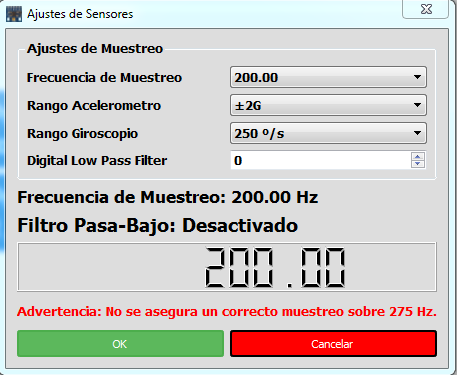
\includegraphics[scale=0.6]{images/AjustesSensores}
  \caption{Ventana Ajustes Sensores}
  \label{fig:ajustessensores}
\end{figure}


\begin{figure}[H]
\centering
  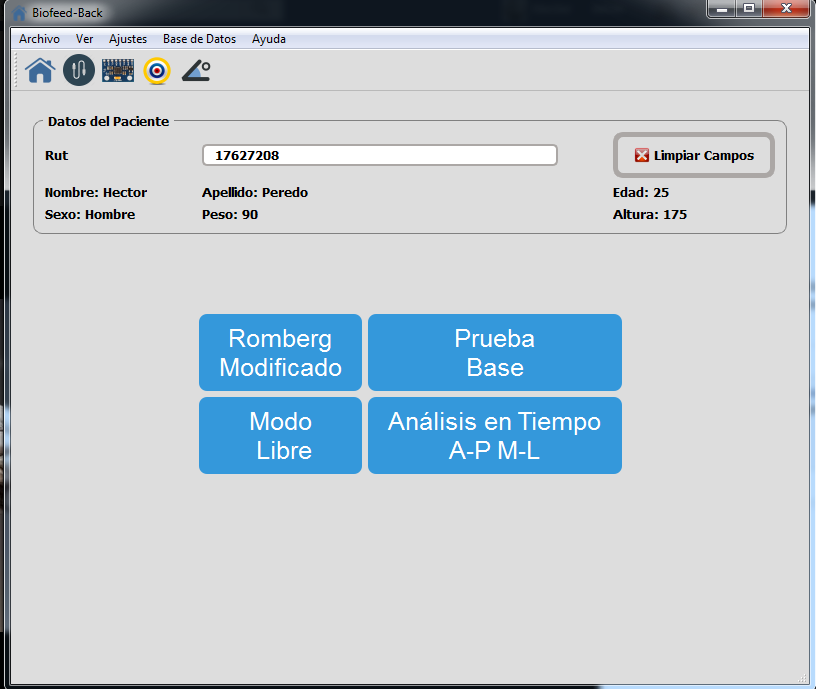
\includegraphics[scale=0.6]{images/mainwindow}
  \caption{Ventana Principal V0.1}
  \label{fig:mainwindow}
\end{figure}

Luego de realizar la conexión de forma exitosa, se procede a desplegar la información obtenida, en forma de gráficos.

\begin{figure}[H]
\centering
  \frame{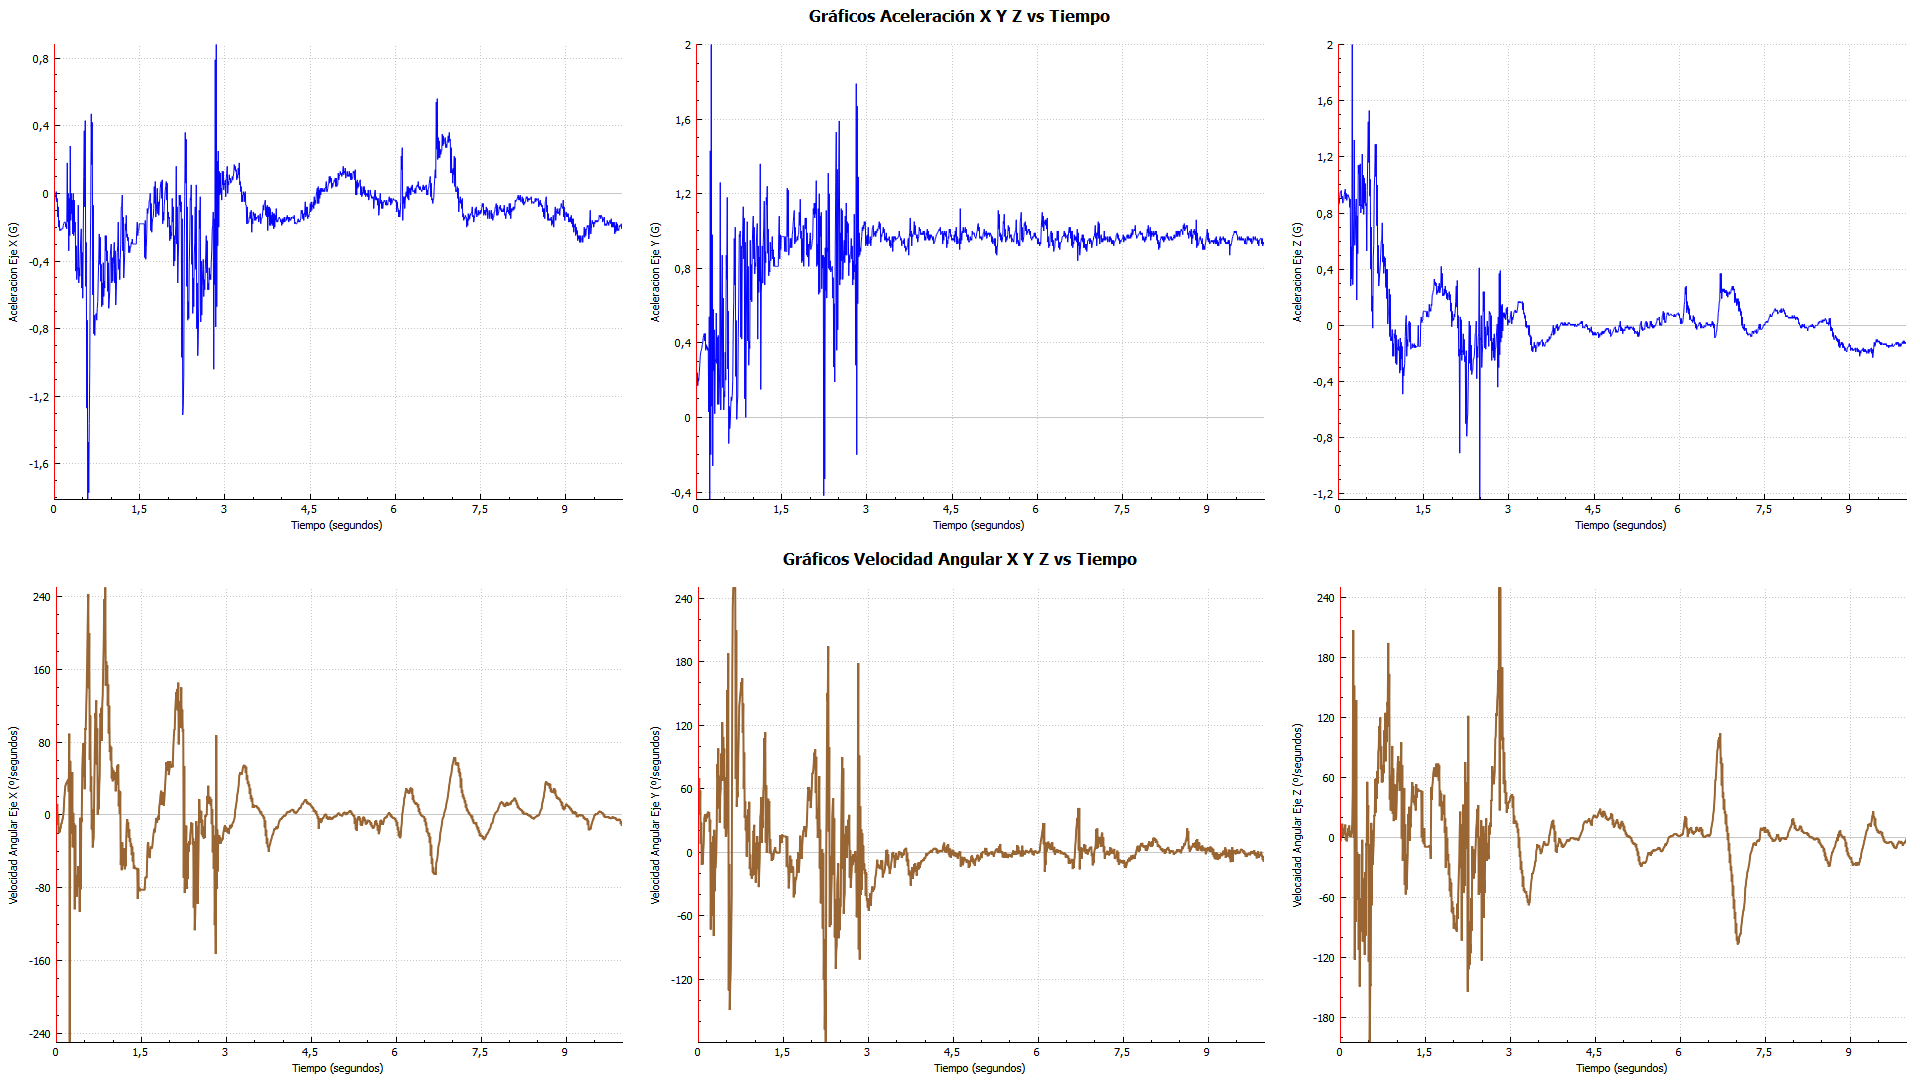
\includegraphics[scale=0.3]{images/graficosensores}}
  \caption{Gráficos de los sensores}
  \label{fig:Graficosensores}
\end{figure}



\subsection{Características}
El software permite configurar la gran mayoría de opciones de tanto velocidades de muestreo, los rangos para la captura de información del movimiento, así como lo que se representaran en pantalla, tamaños de los elementos a graficar, limitar geométricamente el gráfico, entre otros.

Se uso bastante la geometría analítica, para la generación y representación gráfica tanto de los objetivos en las pruebas, como para la intersección del movimiento realizado con cada uno de estos. De igual manera la trigonométrica para limitar el área del movimiento según el radio que sea definido para el examen.

Reportes: Cada uno de los gráficos, los que despliegan las medidas tomadas o los que representan los resultados de el ejercicio, pueden ser almacenados en muestras de cada uno de los gráficos, o también generar una imagen de estos.

Herramientas de Análisis Gráficas: ventanas desplegables acompañadas a un gráfico que permiten de forma interactiva seleccionar partes del gráfico, para analizar intervalos según se estime conveniente y a su vez obtener de este datos como, los valores máximos y mínimos, la media, desviación estándar de los datos, y en el caso del desplazamiento obtener la velocidad media del intervalo analizado.

\begin{figure}[H]
\centering
  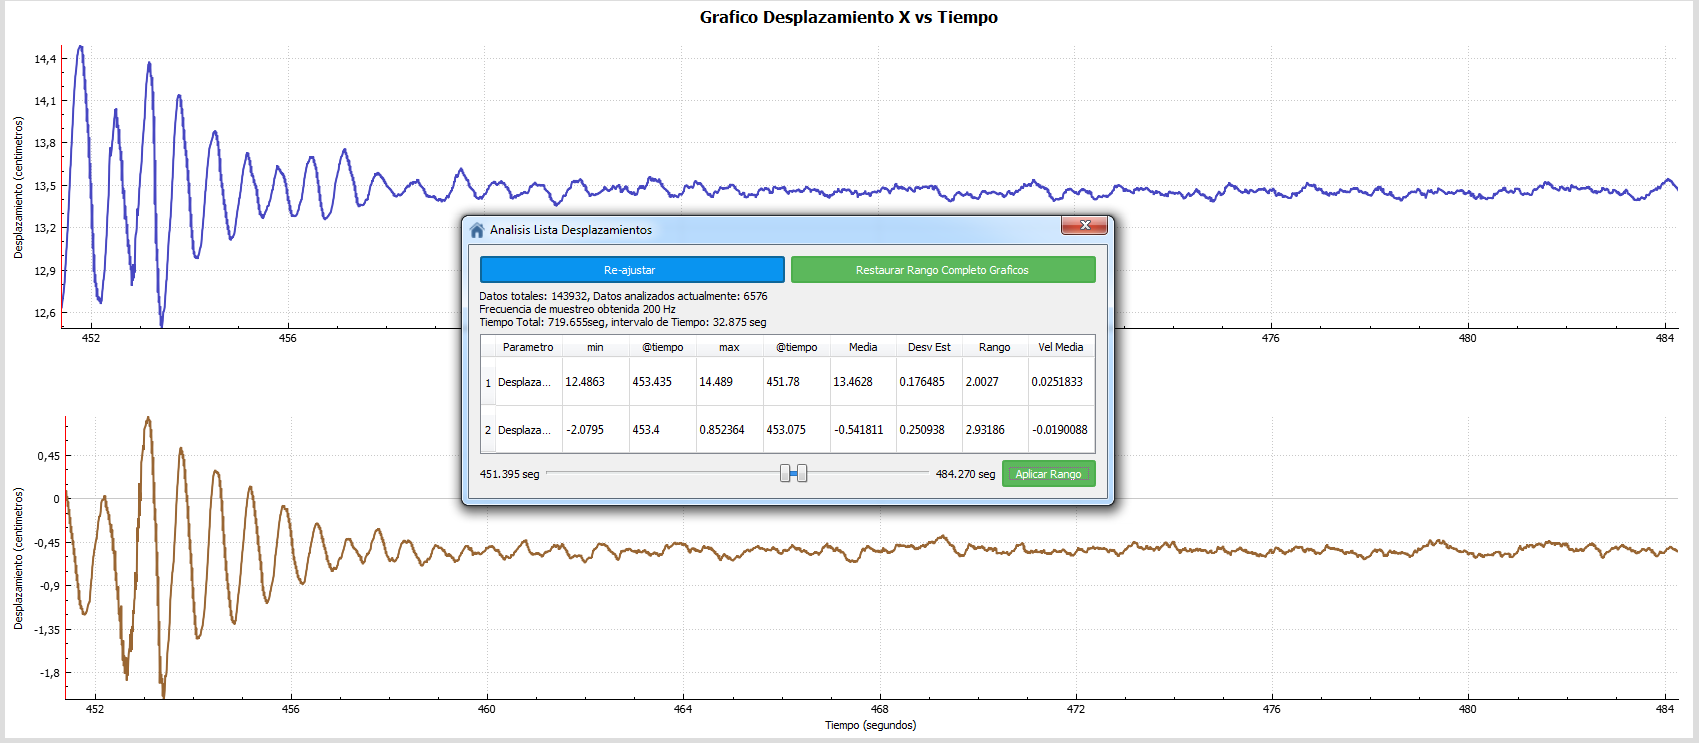
\includegraphics[scale=0.3]{images/analisisGraficos}
  \caption{Ejemplo Herramienta de Análisis}
  \label{fig:analsisGraficos}
\end{figure}

\begin{figure}[H]
\centering
  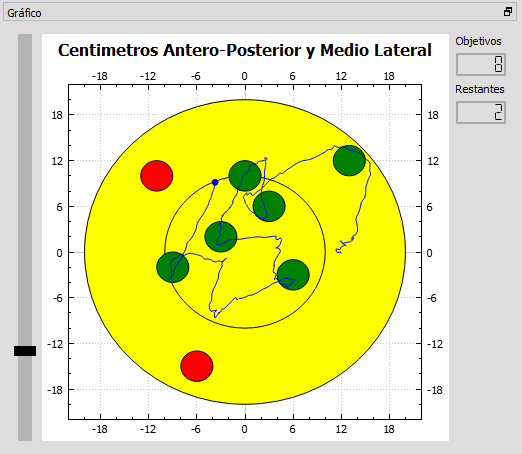
\includegraphics[scale=0.7]{images/graficoPrincipal}
  \caption{Gráfico de Prueba}
  \label{fig:graficoPrincipal}
\end{figure}


\begin{figure}[H]
\centering
  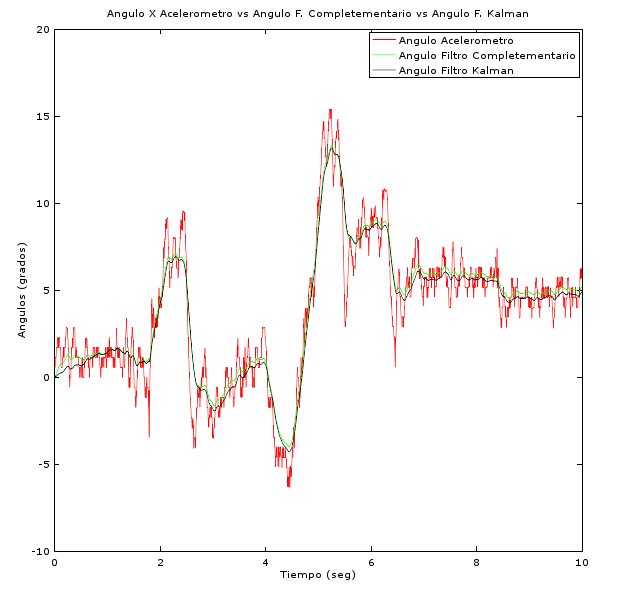
\includegraphics[scale=0.7]{images/angKalCom}
  \caption{Comparativa Angulo Acelerómetro vs Filtro Kalman vs Filtro Complementario}
  \label{fig:AnguloXvsFiltros}
\end{figure}

\subsection{Fusión de Datos Sensores:}
Para el análisis del balance postural se requiere el cálculo del ángulo y para ello se usara la información proveniente de ambos sensores con el fin de obtener el ángulo lo más refinado posible.

\subsection{Cálculo Ángulo con Acelerómetro} Si es utilizado acelerómetro este nos entrega el ángulo exacto pero al ser producida cualquier variación en la aceleración en cualquiera de sus 3 ejes de medición que no sea producto tan solo de la fuerza gravitacional será interpretada como un cambio de rotación, por lo cual se generan medida erráticas debido a los cambios de aceleración constantes que son generados al girar la IMU como se muestra en el ejemplo para el cálculo de los angulos X ver ecuación (\ref{eq:calculoanguloXsensorvertical}) e Y ver ecuación (\ref{eq:calculoanguloYsensorvertical}) usando el sensor en posición vertical.

\begin{figure}[H]
\begin{equation}
anguloX = \tan{\left(\frac{aceleracionX}{\sqrt{aceleracionZ^{2}+aceleracionY^{2}}}\right)}
\label{eq:calculoanguloXsensorvertical}
\end{equation}
\begin{equation}
anguloY = \tan{\left(\frac{aceleracionZ}{\sqrt{aceleracionX^{2}+aceleracionY^{2}}}\right)}
\label{eq:calculoanguloYsensorvertical}
\end{equation}
\end{figure}

\subsection{Calculo Angulo con Giroscopio} 
En cambio , si utilizamos el giroscopio a diferencia del acelerómetro, podemos realizar los cálculos del ángulo con mayor precisión pero al no tener una referencia clara del punto de partida de la mediciones, es difícil de interpretar la información y además con el tiempo los datos comienzan a acumular error, a estos errores acumulados se les conoce como drift o deriva.

\subsection{El Filtro Complementario}

En síntesis tenemos un acelerómetro que entrega ángulos con referencia en la posición del sensor, pero muy susceptible a la variación de cambios de aceleración del IMU y en cambio el giroscopio nos permite calcular el angulo de manera exacta, pero si tener una clara referencia de la posición donde esta el sensor. 

Para unificar la información proveniente de ambos sensores existe un filtro , que nació principalmente de la práctica, conocido como el Filtro Complementario.
El filtro requiere un ángulo de punto de partida y para esto se utiliza el acelerómetro para recoger el ángulo inicial, ya que, al poseer la referencia de la gravedad, se puede tener obtener una mejor estimación para comenzar a realizar las iteraciones del filtro.
\newline
El Filtro complementario es ampliamente usado en unidades inerciales y sistemas de visión. Este filtro es en si es un filtro de Kalman de estado estacionario para una cierta clase de problemas de filtrado.
Esta compuesto por la una unión de dos filtros diferentes:
\begin{itemize}
\item \textbf{Filtro Pasa-Bajo:} Se usa para eliminar las frecuencias altas del acelerómetro, por lo cual dejamos pasar bajo ciertas frecuencias, para eliminar el ruido detectado por el cambio de aceleración (vibración principalmente) en los ejes del acelerómetro.
\item \textbf{Filtro Pasa-Alto:} Se aplica en las mediciones obtenidas por el giroscopio, para eliminar el drift acumulado en el tiempo, dejando pasar solo las de una frecuencia más alta.
\end{itemize}

\begin{figure}[H]
\centering
	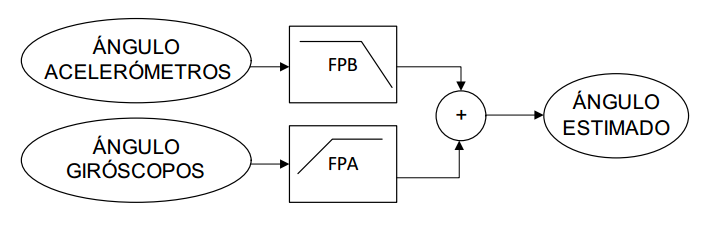
\includegraphics[scale=0.5]{images/FiltroComplementario}
	\caption{Diagrama Filtro Complementario}
    \label{fig:diagramafiltrocomplementario}
\end{figure}

Todo lo anterior queda descrito usando la siguiente Ecuación (\ref{eq:ecuacionFiltroComplementario}):

\begin{equation}
\label{eq:ecuacionFiltroComplementario}
angle = (0.98)*(angle+gyro*dt)+(0.02)*angle\_acc
\end{equation}

En donde cada uno de las variables representa lo siguiente:
\begin{itemize}
\item \textbf{gyro:} Es el ángulo del Giroscopio que hemos calculado previamente.
\item \textbf{angle\_acc:} El ángulo calculado por los datos del Acelerómetro.
\item \textbf{dt:} Corresponde a la variación en segundos desde la ultima vez que se aplico el filtro para calcular el angulo.
\item \textbf{Coeficientes:}  0.98 y 0.02 pueden ser personalizados para aumentar o disminuir la contribución de cada sensor, pero se debe tener en consideración que la suma de ambos debe ser 1.
\end{itemize}

\subsection{Filtro de Kalman}

\subsection{Calculo de la proyección del Ángulo}
 Usando el principio que la posición bípeda-quieta puede ser representada como un péndulo invertido, por lo tanto es aplicable la trigonometría para la obtención del desplazamiento proyección generada a partir de una variación en el ángulo, esta variación angular es directamente proporcional a el desplazamiento en el eje horizontal, seria de una forma simple, tomando la distancia a la que fue puesta el sensor como la hipotenusa de un triángulo rectángulo, como se muestra en la Figura (\ref{fig:proyeccion}), al aplicar la función $\sin$ del ángulo obtenido en grados mediante el uso filtro Complementario, junto con ponderar el valor obtenido por la altura $h$ en la que fue ubicado el dispositivo (hipotenusa del triángulo) , obtendríamos la distancia $d$ en la cual su unidad de medida es la misma usada para describir la altura $h$.
 
 \begin{figure}[H]
\begin{equation}
\label{eq:proyeccion}
d=\sin(\alpha)
\end{equation}
\end{figure}

  \begin{figure}[H]
  \centering
      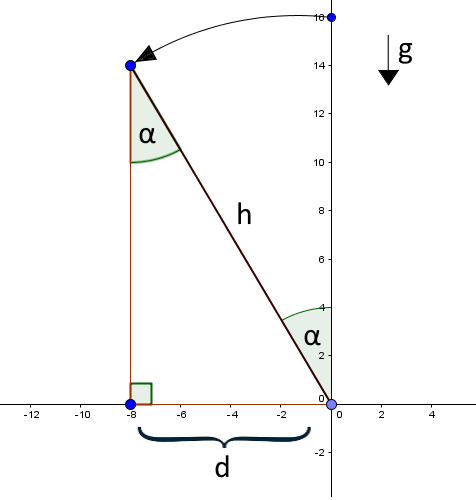
\includegraphics[scale=0.5]{images/calculoProyeccion}
      \caption{Ejemplo calculo proyección Angulo}
      \label{fig:proyeccion}
  \end{figure}

\section{Conclusiones y Trabajos Futuros}
\subsection{Conclusiones}
\subsection{Trabajos Futuros}

\section{Bibliografía}

\printbibliography[heading=none]%Imprimir las referencias

\thispagestyle{empty}
\pagebreak
\newpage

\end{document}